\chapter{Architecture}
\label{chap:architecture}

%This is our webapps Architecture   (3-6 pages)
%\begin{itemize}
%\item  Overall system architecture, short description of main components
%\item  Assessment of strength and weaknesses of chosen %\item  Discussion of alternative technical solutions
%\end{itemize}

\section{Overall system arcitecture}
\label{sec:overallArc}
The system is developed mainly in Angular 2\cite{Angular2:online} and the frameworks does provide a great standard way of developing web-pages. Our system uses the architecture as described on the official website, with some alterations. Angular 2 is using the software architecture of MVC \cite{Angular2:online} where each component consists of a separate HTML view and a component class with decorator for defining the controller and model. It is both MVC and modular because of this and we use this to its full extend in our application. 

%we might need to use visio or something to draw thiS :D

\begin{figure}[h]
  \centering
  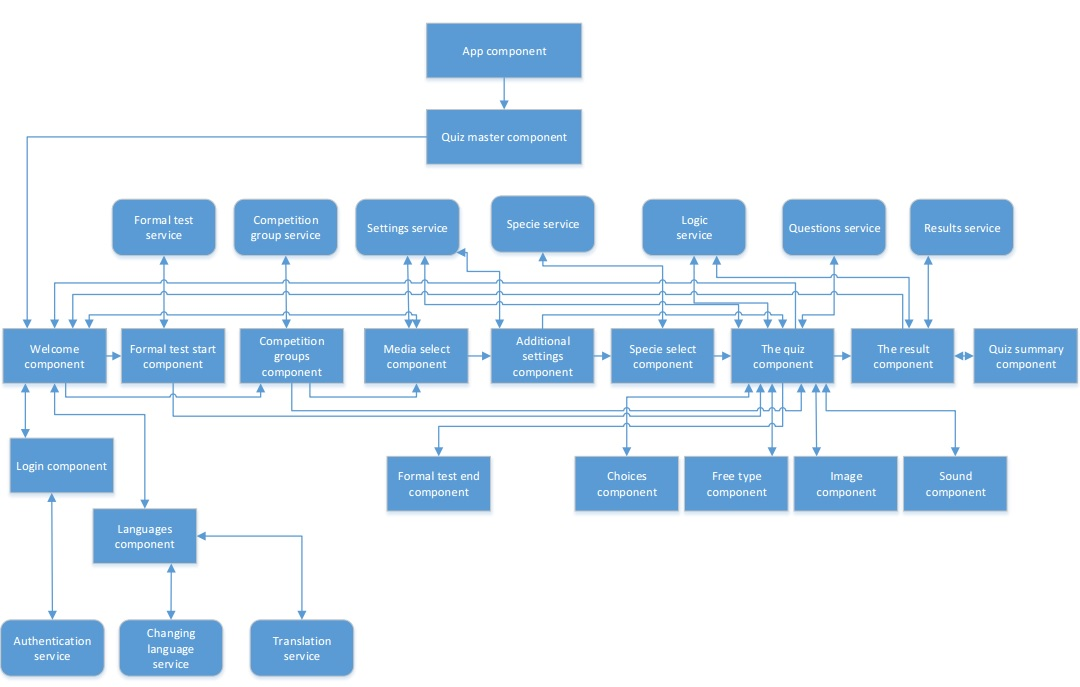
\includegraphics[width=1.0\textwidth]{figures/system_architecture.jpg}
  \caption[Hierarchy]{System architecture}
  \label{fig:Hierarchy}
\end{figure}

Everything starts at the top with bootstrapping the main component, the app component. This component is only in charge of defining the routing for the application and then handing control over to its only child, the quiz master component. This is the boss/god of the application. Here all the services are started and initialized. The next thing to happen is that the loading graphics is replaced with the router outlet, defined in the parent, and the quiz app can start. It all then start at the beginning with the welcome component (not shown above) where the user can select between quiz, competition groups and formal test. Each of the next steps through a quiz uses the routing for switching the main component in focus and using services for both saving data between components and handling communication to the backed API.

Each normal quiz consist of several defined steps with one or more corresponding component. After selecting both the quiz and for example images then the user can input several additional parameter for he quiz like the area and difficulty level. These are defaulted to the most popular choice based on previous testing. All of these settings are then promptly saved in the quiz settings service which is all knowing about the state of the quiz, but does no processing or server communication. Then the quiz will start on the next step and the correct sub components will be loaded. For example the image component if an image quiz and the sound component if a sound quiz was chosen. Then the quiz question service retrieves a quiz from the API and sends it to the quiz logic service for processing. Each question is then contained in a quiz question objects which holds every peace of knowledge associated with that question. The reason for this is because later it can support  multiple questions in one (like in several sound quiz) with the rest of the application treats it as a single question. Once the quiz is over it will allow the user (if hints were not used) to submit score to server using the results service. Optionally, if they are logged in it will submit their results anyways for the user quiz statistic function on the server.

The formal test works a bit different. First off it requires an access code/token provided when your application is approved. Then the API does NOT return information about the choices and right answer to the question. It also does not return any usable media URL, just a one time token that can be exchanged once for the image. It also forces the users to do the free type where they have to select the correct specie from a list of all species. It also skips the in-between question part, giving no breaks. At the end it submits the response to the server, allowing examiners to grade the test. 

The last part in the competition group where people can compete inside a group with its own set of rules, limited amount of attempts, access codes and its own high score list. Can be used by anyone from friends to school classes. Once selected and clicked play it will go directly to the quiz with all settings stored if it has restrictions. Some groups have no restrictions, just having all high score submitted together. The login/authentication is entirely server side as client side security is no security. It offers the possibility of registering, login and resetting password. It also enables autologin and grating authenticating tokens and refresh tokens. There are some more features like  changing language, bit that is mostly self explanatory. 
%shall we mention that the group does not neccecary need to have pre defined settings?


The backend API will not be thoroughly documented as it is make mostly outside the scope of this project and it is not open source. Some documentation will be provided however, for example the API endpoints used by the quiz. The back-end is written in PHP 7 and is using MySQL. Most of the functionality used by the quiz already existed at the beginning of the project, at the already existing flash application but was using XML, not JSON. This was a problem since Angular 2 really favours JSON and it been more lightweight, as well as easier to work with in JavaScript/TypeScript. Some additional API's were added, for example the competition group listing. Throughout the development process some bugs were discovered in the old API  and were fixed, resulting  the already existent API benefiting from this project as well. 


\section{Strength and weaknesses of chosen technologies}
\label{sec:stregthandwic}
Most, if not all of the chosen technologies for this projects is cutting edge and some, like Angular 2 just being  barely in realise candidate level at the end of the project. We debated a lot over the choice between Angular 1 and 2. It boiled down to either continuing on a dying platform with great documentation and extensive knowledge base across the Internet including blog post and problems solved on stack overflow or venturing into the new and unknown. Angular 2 did however has too many new and exiting functionality for us to pass it up and we quickly learned how much easier Angular 2 is to use than Angular 1. In retrospective it almost seems like Angular 1 is just a prototype for what to come. Using a tutorial on Udemy \cite{TheCo73:online} we managed quickly to learn the new framework and start working. The modular approach of the framework greatly benefited the team as each person could work on there own component in parallel with the rest.

When it comes to great web design it is not really a debate on which framework to use. Bootstrap is the way to go. We debate a bit about using the new Bootstrap 4, but as it only was in alpha. We felt it was a bit too new and unstable for our project and decided to use the latest Bootstrap 3 with great success. The framework/design template worked wonderfully for a group with no designer as it let us create relative amazing looking quiz with little effort. It also handles responsiveness amazingly which is a big part of making a quiz which both work on desktop, tablets and mobile.

We also selected Sass\cite{Sass:14:online} over CSS for extra functionality, even if we did not really use all of it. If offers a lot of extra functionality not provided by plan old CSS, but is is just extending like TypeScript is extending JavaScript. It means we could always fall back on CSS if we did not know the correct Sass way of doing something. 

Another important choice was choosing Gulp for our automation tool as our previous automation tool as Grunt seemed to be dying. As a side note we do not really believe that gulp will live long either, but there is not greater tool right now. It is really easy to learn (and drop lather) offering most required functionality via plug-ins made by the community.

Selecting so many new technologies at the same time made it a lot more challenging to get started as we had to learn every new technology at the same time in parallel. This was one of the reasons we used a test repository the first sprint to test and learn everything before moving onto the real repository. Might be worth mentioning we used git and GitHub for version control as both greatly improve collaboration on coding projects, and makes it easier to blame the right person when it breaks.

\section{Alternative technical solutions}
\label{sec:alttec}

There are a lot of great alternatives to what we have chosen for this project. The choices was mostly in front-end since the back-end was already developed. The most important, Angular 2 could have been replaced with Angular 1, but it is a inferior framework. Angular 2 is improved on every area as well as somewhat forcing (or strongly encroaching) the use of TypeScript. All team members used Angular 1 in the last semester's project and all of us see a clean benefit with Angular 2. Other choices was jQuery and React, but both of them have the downside of just adding some JavaScript to the HTML documents, unlike Angular 2 which does it the other way around and take full control, for example jQuery is mostlly usefully for just adding some extra functionality to a website, not making a JavaScript application as Angular 2 is allowing us. React also has some great benefits, but it is rather strict in the sense that it can not be used for anything that can potentially compete  with Facebook, as they made it. We like no restrictions and therefore we dropped it, even if it can do a lot of amazing things.

%I guess decribe what angular 1 is and react + grunt and normal css?